\question Give a formulation of the \emph{Rush Hour Problem},
where we want to get our car to the exit using as few moves as possible, 
as a ‘global path-based’ search problem. 
How might your formulation change if all you were interested in was: 
minimizing the number of moves of your car; 
or minimizing the total number of lorry moves?

\question Which data structures might you use in your formulation of the \emph{Rush Hour Problem} in question 1? Outline how you might describe your state transitions in terms of these data structures?

\question Give another formulation of \emph{TSP} as a `global path-based' search problem where the formulation is similar to \emph{TSPi} except that now in a state transition from some state $x$ you are allowed to `insert' an unvisited city (from the $n$ cities in total) somewhere in the list corresponding to $x$;
so, if the list corresponding to $x$ has $i$ members,
where $1 \leq i \leq n - 1$,
there are $i + 1$ `insertion points' where the new city might be inserted.
You should ensure that all step-costs are non-negative.

\question Give a formulation of the \emph{Disjoint Connecting Paths Problem}, where you wish to minimise the sum of the lengths of the eventual paths, as a `global path-based' search problem. How might your formulation change if all you were interested in was minimising: 
\begin{enumerate}
    \item the length of the path of person $p_1$;
    \item the length of the path of person $p_1$ minus the length of the path of person $p_2$ but so that this value is non-negative;
    \item the number of synchronised rounds of moves of persons?
\end{enumerate}

\question Outline how you might formalise the problen of solving \emph{Rubik's Cube}, using as few moves as possible, as a `global path-based' search problem.

\question Consider the maze in Figure \ref{fig:maze}. 
Think of the maze as occupying a $29 \times 29$ grid, within the outer walls, where each grid-cell is either free-space (white cells) or an impenetrable concrete wall (grey cells).
The entrance is through the top wall at the far left and the exit is through the bottom wall at the far right.
Explain how you can precisely formulate the problem of moving from the entrance to the exit, 
as quickly as possible, 
as a `global path-based' search problem.
You should assum,e that the actions available to your agent are `face-north', `face-south', `face-east', `face-west', and `move-$n$-steps', where $1 \leq n \leq 28$ (in the direction you are facing). If an action `move-$n$-steps' is applied which forces the agent to bump into a wall then the agent does just this and ends up concussed (which is to be avoided!).

\begin{figure}
    \centering
    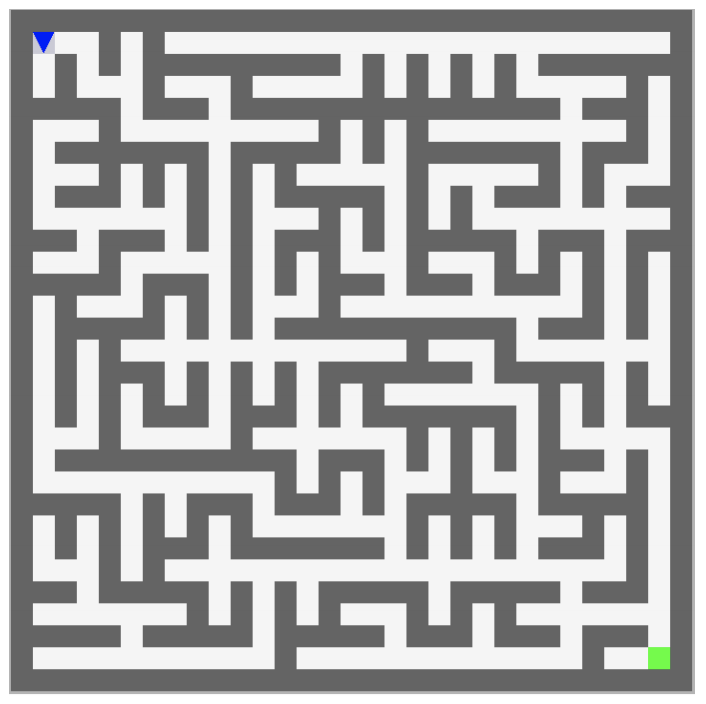
\includegraphics[width = 0.4\textwidth]{images/maze.png}
    \caption{A maze.}
    \label{fig:maze}
\end{figure}

\question Suppose that there is a collection of houses that need painting and that some pairs of houses are related by being neighbours of each other.
Between any two neighbouring houses there is a path that directly joins the two houses, with these paths having various lengths.
Jimmy has been hired to paint the houses so that neighbouring houses must be painted with different colours.
Moreover, Jimmy has to paint the houses as cheaply as possible: the time he spends walking from house to house costs money as does the number of tins of paint he buys.
However, Jimmy buys paint `by the colour' so that if he buys one tin of red paint then he gets an unlimited supply of red paint.
Jimmy starts at the gate to the complex of houses (there are paths from the gate to some of the house). 
Formalise the problem of painting all the houses so as to minimise Jimmy's costs as a `global path-based' search problem. 

\question The \emph{Knapsack Problem} is defined as follows: an input is a set of $n$ items, each of which has a weight and a cost which are both positive intevers, 
together with a knapsack that can hold a total given weight $b$ of items;
and an output is a set of items of greatest cost so that these items fit in the knapsack 
(that is, the sum of their weights is at most $b$). 
Show how the Knapsack Problem can be formulated as a `global path-based' search problem.
What does a path in your state space correspond to?

\question The \emph{Water Jug Problem} is defined as follows.
There are two jugs, the first of which holds $4$ litres and the second of which holds $3$ litres.
Neither jug has any measurements marked on it.
There is a pump that can be used to add water to either of the jugs.
The aim is to get exactly $2$ litres of water into the $4$ litre jug.
Formulate the \emph{Water Jug Problem} as a `global path-based' search problem and give a solution.
You should justify your abstraction.
Draw the search tree so as to include tree-nodes up to depth $2$.

\question Consider the following abstractions of real world problems and comment on whether they are suitable abstractions.
\begin{parts}
    \part We are given tables of pairs of source and destination locations for each of the modes of transport `walk', `car', `bus', `train', and `plane'. 
    For each source-destination entry in each table, there is a value for the time taken to get from the source to the destination 
    (there may be more than one entry for a given source-destination pair in a table,
    e.g., there may be two different routes to drive by car from location $u$ to location $v$,
    with different times).
    Our aim is to get from location $u_0$ to location $v_0$ as quickly as possible.
    \begin{enumerate}
        \item states: the various locations;
        \item actions: `move';
        \item transitions: if a source-destination pair $(u, v)$ appears in some table then there is a transition from $u$ to $v$ under action `move';
        \item initial state: location $u_0$;
        \item goal states: location $v_0$; and
        \item step-costs: if there is a transition $(u, move) \mapsto v$ then the step-cost is $t$ where $t$ is the time taken to get from $u$ to $v$.
    \end{enumerate}

    \part We are trying to solve the \emph{$8$-Puzzle Problem}.
    \begin{enumerate}
        \item states: the start configuration start and the end configuration end;
        \item actions: `move';
        \item transitions: there is one transition from start to end;
        \item initial state: start;
        \item goal states: end; and
        \item step-costs: the transition from start to end under action `move' has step-cost 1.
    \end{enumerate}

    \part We are trying to solve the \emph{Water Jug Problem}.
    \begin{enumerate}
        \item states: all possible pairs $(u, v)$ where $u$ and $v$ are non-negative real numbers;
        \item actions: `pour' and `fill';
        \item transitions: from state $(u, v)$, there is a transition under action `pour' to state $(u', v')$ and to state $(u'', v'')$ where $u - u' = v' - v > 0$ and $u'' - u = v - v'' > 0$; and from state $(u, v)$ under action `fill' there is a transition to state $(u + x, v + x)$, for each non-negative real number $x$;
        \item initial state: $(0,0)$;
        \item goal state: $(2, 0)$; and
        \item step-costs: every transition has step-cost $1$.
    \end{enumerate}
\end{parts}

\question Give a necessary and sufficient condition on a search problem that ensures that the search tree is infinite.

\item In the second formulation of \emph{TSP} in the lecture notes, namely \emph{TSPii}, how might you define step-costs and actions?
